\documentclass[fontsize=10pt,paper=b5,open=any,
twoside=no,toc=listof,toc=bibliography,headings=optiontohead,
captions=nooneline,captions=tableabove,english,DIV=15,numbers=noenddot,final,parskip=half-,
headinclude=true,footinclude=false,BCOR=0mm]{scrartcl}
\pdfvariable suppressoptionalinfo 512\relax
\synctex=1

\author{Valentin Boettcher}
\usepackage{hirostyle}
\usepackage{hiromacros}
\addbibresource{references.bib}
\acsetup{
  make-links = true ,
  format = \emph ,
  list / display = all ,
  pages / display = all
}
\DeclareAcronym{mlong}{short=LTAD, long=long-time time-averaged mean displacement}
\DeclareAcronym{rwa}{short=RWA, long=Rotating-Wave Approximation}

\title{The non-Markovian Quantum Walk for Finite Baths}
\date{2023}
\graphicspath{{plots}}

\usepackage{keyval}
\usepackage{xparse}

\setkeys{Gin}{width=\linewidth,totalheight=\textheight,keepaspectratio}
\makeatletter
\define@key{hirodims}{width}{\def\hiro@width{#1}}
\define@key{hirodims}{scale}{\def\hiro@scale{#1}}

\NewDocumentCommand\includeplot{O{width=\linewidth} m o}{%
  \begingroup
  \setkeys{hirodims}{width=\expandafter{\linewdith},scale=1,#1}% the
  % current values
  \includegraphics[width=\hiro@scale\hiro@width]{plots/#2}
  yoo\the{\Gin@width}
  \endgroup
}
\makeatother

\begin{document}
\maketitle
\tableofcontents


\section{Introduction}
\label{sec:introduction}
The aim of this document is to try to reproduce the results of
\cite{Ricottone2020} for a finite sized bath with non-vanishing
coupling strength. As the phase transition observed in
\refcite{Ricottone2020} is non-analytic, we expect some finite-size
effects that wash out the transition. Nevertheless, a qualitatively
similar behavior should be observable.

In \cref{sec:model} the basic model is briefly introduced and
\cref{sec:mean-displacement-1} discusses the observable of interest to
us. In summary, the observable of interest is the (long-time-averaged)
mean displacement \(\ev{m}\) of a particle on an SSH lattice with
extra energy levels (henceforth called the bath) attached to each unit
cell. Depending on the nature of the couplings to these extra levels
one finds~\cite{Ricottone2020} that this observable takes on universal
values depending on the toplogical phase of the SSH
chain\footnote{More precisely reference SSH chain without detuning of
  the site energies and without the extra bath levels.}. This leads to
a two dimensional phase diagram, where one dimension is the model
parameter of the SSH chain and the other axis is related to the bath
structure.

\Cref{sec:Born-approximation} revisits the results of
\refcite{Ricottone2020} by briefly describing the solution of the
model using a perturbative approach, but without taking the continuum
limit. The detailed analysis of the resulting expression is postponed
to a later point (\cref{sec:criterion-bath-size}).

As the numerics indicated, that the approximation assumed in
\cref{sec:Born-approximation} is too restrictive in a setting with
finitely many bath states and finite coupling strength, an exact
solution is used to indicate a method to counter the effects of the
finite coupling strength in \cref{sec:exact-solution}. While
relatively weak coupling is still required, the vanishing coupling
that the Born approximation would require is not necessary in this
case.

\Cref{sec:strong-coupl-limit} discusses the limit of ultra-strong
coupling, where \(\ev{m}\) takes on a different universal value than
in the weak coupling case, irrespective of the bath structure.

In \cref{sec:criterion-bath-size} we present an analytic criterion for
the size of the bath that would be required to see the universal
behavior of \(\ev{m}\) for a specific bath
structure. \Cref{sec:mean-displacement} highlights how the results of
the previous sections may be used to construct the phase diagram for a
finite sized system.

Examples of the resulting phase diagrams resulting from exact
numerical calculations are presented in \cref{sec:phase-diagram}.


\subsection{Model}
\label{sec:model}

We will discuss how the behavior of the model introduced in
\refcite{Ricottone2020} for the limit of weak coupling and an infinite
bath may be reproduced with both finite coupling strength and a finite
number of bath levels.

The model Hamiltonian is that of an SSH-Chain~\cite{Su1979} with a
number of bath states coupled to each unit cell \(H=H_{A}+H_{\bar{A}}+V\)
\begin{align}
  \label{eq:36}
  H &= H_{A} +H_{\bar{A}} + V\\
  H_{A} &= ∑_{m}ω_{A} \ketbra{A,m} \\
  H_{\bar{A}} &= Σ_{m}(ω_{A} + ω)\ketbra{B,m}+
                   ∑_{j}\bqty{ω_{j}\ketbra{j, m} + g_{j}
                   \pqty{\ketbra{j,m}{B,m} + \hc}}\\
  V&=∑_{m} v\pqty{\ketbra{A,m}{B,m} + u\ketbra{A,m}{B,m+1} + \hc},
\end{align}

In momentum space, the model Hamiltonian takes the form \(H=H_{A}(k) +
H_{\bar{A}}(k) + V(k)\) with
\begin{align}
  \label{eq:35}
  H_{A}(k) &= ω_{A} \ketbra{A,k} \\
  H_{\bar{A}}(k) &= (ω_{A} + ω)\ketbra{B,k}+
                   ∑_{j}\bqty{ω_{j}\ketbra{j, k} + g_{j}
                   \pqty{\ketbra{j,k}{B,k} + \hc}}\\
  V(k)&=\abs{v(k)}\pqty{\eu^{\iu ϕ(k)}\ketbra{A,k}{B,k} + \hc}
\end{align}
with \(v(k) = \abs{v (1+u\eu^{\iu k})}\).

Upon eliminating the \(B\) site from the above through a
Schrieffer-Wolff transformation for \(ω\gg v(k)\), we end up with
\begin{equation}
  \label{eq:37}
  H(k) = \tilde{ω}_{A} \ketbra{A,k} + ∑_{j} \bqty{\tilde{ω}_{j} \ketbra{j, k}
    + \pqty{\tilde{η}_{j}\ketbra{A,k}{j,k} + \hc}},
\end{equation}
where the
\(\tilde{η}_{j}(k) \sim \tilde{η}_{j}(0) \frac{v(k)}{v(0)}\). The
tildas signify quantities renormalized due to the Schrieffer-Wolff
transform and will be dropped in the following.


One final technicality is, that \(u\) influences the overall coupling
strength and therefore the behaviour of the model. Therefore we
normalize \(v(k)\) so that \(v (1+u) = v + v\prime\) remains constant
with respect to \(u\) which is in accordance with
\refcite{Rudner2009}.

\subsection{Mean Displacement}
\label{sec:mean-displacement-1}

The \emph{mean displacement} is defined as
is the mean displacement
\begin{equation}
  \label{eq:59}
  \ev{m(t)} \equiv ∑_{m}m {ρ_{\bar{A},m}(t)}
\end{equation}
where
\(ρ_{\bar{A},m}(t) = {∑_{l\neq A} \abs{\braket{l,m}{ψ(t)}}^{2}}\) is
the probability that the walker does not reside on the \(A\) site in
cell \(m\) at time \(t\).

As the quantity \(\ev{m(t)}\) can fluctuate in time and we will be
interested in long-time beahavior, we additionally define
\begin{equation}
  \label{eq:39}
  \ev{m} \equiv \lim_{T\to ∞} \frac{1}{T}∫_{0}^{T}\ev{m(t)} \dd{t}
\end{equation}
which we will refer to as \ac{mlong}.

In momentum space this becomes
\begin{equation}
  \label{eq:40}
  \ev{m} = ∫_{0}^{2π}(1-ρ_{A})\pdv{ϕ(k)}{k} \frac{\dd{k}}{2π}
\end{equation}
with
\begin{equation}
  \label{eq:41}
  ρ_{A}(k) = \lim_{T\to ∞}\frac{1}{T} ∫_{0}^{T}ρ_{A}(t, k)\dd{t} = \lim_{T\to
    ∞}\frac{1}{T} ∫_{0}^{T}\abs{\braket{A,k}{ψ(t)}}^{2}\dd{t}.
\end{equation}

\section{Results using the Born Approximation}
\label{sec:Born-approximation}

In the limit of very weak coupling we can solve for \(ρ_{A}\) in terms
of a non-Markovian master equation by employing perturbation theory to
second order\footnote{Which is the first nontrivial order} in the
coupling \(V\).
\begin{equation}
  \label{eq:42}
  \dot{ρ}_{A}(k,t) = ∫_{0}^{t}Σ(k, t-t\prime) ρ_{A}(k, t\prime)
\end{equation}
with the self-energy
\begin{equation}
  \label{eq:43}
  Σ(k,t)=-2 ∑_{j}\abs{η_{j}(k)}^{2}\cos((ω_{k}-ω_{A})t)
\end{equation}
with \(j=\overline{1,N}\).

We are interested in the long time average of \(ρ\) which can be
expressed as
\begin{equation}
  \label{eq:44}
  {ρ}_{A}(k)=\lim_{T\to
    ∞}\frac{1}{T}∫_{0}^{∞}\eu^{-\frac{t}{T}}ρ_{A}(k,t)\dd{t} =
  \lim_{s\to 0} s \tilde{ρ}_{A}(k, s) = \eval{\bqty{\dv{s} \frac{1}{\tilde{ρ}_{A}(k,s)}}^{-1}}_{s=0}
\end{equation}
where \(\tilde{ρ}_{A}({k, s})\) is the Laplace transform of \(ρ_{A}(k,
t)\).

The equation of motion \cref{eq:42} gives direct access to
\(\tilde{ρ}_{A}\)
\begin{equation}
  \label{eq:45}
  \tilde{ρ}_{A}({k, s}) = \frac{ρ_{A}(k,0)}{s - \tilde{Σ}(k, s)} = \frac{1}{s - \tilde{Σ}(k, s)},
\end{equation}
with
\begin{equation}
  \label{eq:46}
  \tilde{Σ}(k, s) = -2 ∑_{j}\abs{η_{j}}^{2} \frac{s}{s^{2}+(ω_{j}-ω_{A})^{2}} =
  -∑_{j}\abs{η_{j}}^{2} \bqty{\frac{1}{s+\iu (ω_{j}-ω_{A})} + \frac{1}{s-\iu
      (ω_{j}-ω_{A})}}.
\end{equation}

Using \cref{eq:44} and setting \(ω_{A}=0\), this yields
\begin{equation}
  \label{eq:47}
  ρ_{A}(k) = \frac{1}{1 + 2∑_{j}\frac{\abs{η_{j}}^{2}}{ω_{j}^{2}}} =
  \frac{1}{1+2 U_{A}}.
\end{equation}

We now assume that the \(η_{j}\) are chosen so that in the continuum
limit \(N\to ∞\)
\begin{equation}
  \label{eq:48}
  ∫_{0}^{∞}f(ω)∑_{j}\abs{η_{j}}^{2} δ(ω-ω_{j})^{2}\dd{ω} =
  ∫_{0}^{∞}J(ω) f(ω)\dd{ω}
\end{equation}
for arbitrary (smooth) functions \(f\), where \(J\) is called the
spectral density. We make the model assumption
of an ohmic-type spectral density
\begin{equation}
  \label{eq:49}
  J(ω) = \frac{\abs{v(k)}^{2}}{\abs{v(0)}^{2}} g_{0}^{2}\frac{α+1}{ω_{c}^{α+1}}
  \begin{dcases}
    ω^{α} & \mathrm{if}\, ω \leq ω_{c},\\
    0 & \mathrm{otherwise}.
  \end{dcases}
\end{equation}
For \(α<(>)1\) this we call \(J\) a sub(super)-Ohmic spectral density,
whereas for \(α=1\) we have an Ohmic spectral density. Let us define
\(J_{α}=g_{0}^{2}\frac{α+1}{ω_{c}^{α+1}}\) for convenience.


The \(ω_{j}\) and \(η_{j}\) may be chosen according to
\cref{sec:discretization-bath}.

In the continuum limit \(U_{A}\to ∞\) for \(α\leq 1\) and remains finite
for \(α>1\), which leads to the \ac{mlong} \(\ev{m}\) having a sharp
transition from \(0\) to \(1\) for \(α\leq 1\) which becomes washed
out for \(α>1\).

We wish to study how this limit is approached with a finite bath and
in finite times. The Born approximation requires that \(η\to 0\)
sufficiently fast for \(N\to ∞\) so that the resulting long timescale is
unlikely to be resolved experimentally.

\section{Exact Solution}
\label{sec:exact-solution}

Numerics (see \cref{fig:unshifted_overview}) at finite coupling
strengths suggest that the behavior for the weak coupling limit may
not be naively reproduced in this setting.

\begin{figure}[htp]
  \centering
  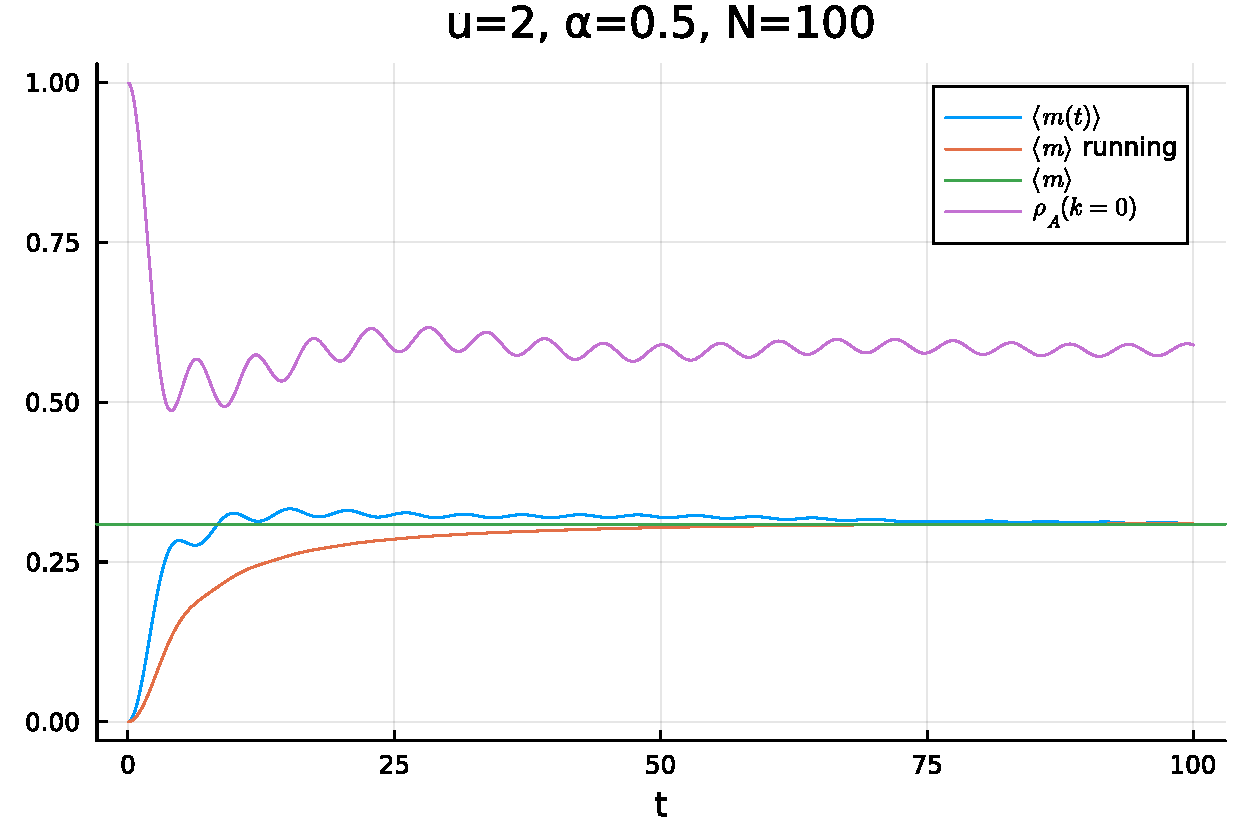
\includegraphics[width=.8\linewidth]{plots/overview_unshifted.tikz}
  \caption{\label{fig:unshifted_overview} A numerical simulation for
    \(g_{0}=10^{-1}\). The mean displacement takes on some
    non-universal value and \(ρ_{A}\not{\to} 0\).}
\end{figure}

In the following we will suppress the \(k\) dependence of the
couplings \(η_{j}\).  Perturbation theory suggests that the energy of
the \(\ket{A}\) state changes according to a lamb shift
\begin{equation}
  \label{eq:1}
  ω_{A} \to ε_{A}^{(2)} = ω_{A} - ∑_{j} \frac{\abs{η_{j}}^{2}}{(ω_{j}-ω_{A})},
\end{equation}
which would make the system insensitive to the spectral density at
\(ω = 0\) unless corrected for.

Let us proceed by writing down the equations of motion for the
coefficients of a general state \(\ket{ψ} = α\ket{A} +
∑_{j}β_{j}\ket{j}\) following from \cref{eq:37}
\begin{equation}
  \label{eq:2}
  \begin{aligned}
    \iu \dot{α} &= ω_{A}α + ∑_{j} η_{j} β_{j} & \iu \dot{β}_{j} = η_{j}^\ast α
                                       + ω_{i} β_{i}.
  \end{aligned}
\end{equation}
Transforming the \(β_{j}\) into a rotating frame with respect to the
\(ω_{i\neq A}\) so that \(\tilde{β}_{i}=β_{i} \eu^{\iu ω_{i}t}\) we obtain
\begin{equation}
  \label{eq:3}
  \begin{aligned}
    \iu \dot{α} &= ω_{A}α + ∑_{j} η_{j} \tilde{β}_{j}\eu^{-\iu ω_{j}t}
    & \iu \dot{\tilde{β}}_{j} = η_{j}^\ast α \eu^{\iu ω_{j} t}.
  \end{aligned}
\end{equation}

The equations for the \(\tilde{β}_{j}\) can be integrated straight forwardly
to obtain \(\tilde{\beta}_{j} = -\iu η_{j}^{\ast} ∫_{0}^{t}\eu^{\iu ω_{i} τ}
  α(τ) \dd{τ}\) which can be substituted into \cref{eq:3} to find a
  closed equation for \(α\)
\begin{equation}
  \label{eq:4}
  \dot{α} = -\iu ω_{A}α - ∫_{0}^{t} Κ(t-τ)α(τ) \dd{τ}
\end{equation}
with \(Κ(t-τ) = ∑_{j} \abs{η_{j}}^{2} \eu^{-\iu ω_{i}
  (t-τ)}\). Laplace transforming both sides of \cref{eq:4} leads us to
\begin{equation}
  \label{eq:5}
  \begin{aligned}
  \tilde{α}(s) &= \frac{α(0)}{s+\iu ω_{A} + \tilde{Κ}(s)} &
     \tilde{Κ}(s) &= ∑_{j}\frac{\abs{η_{j}}^{2}}{s + \iu ω_{j}},
  \end{aligned}
\end{equation}
which is very similar to \cref{eq:45}, save for the explicit
appearance of \(\iu ω_A\). As \cref{eq:45} is related to a probability, it
is real-valued and always has a pole at \(s=0\) independent of
\(ω_{A}\).

A thorough analysis of the above problem can be found in
\refcite{Gaveau1995}. We will limit the discussion to the relevant cases
here.

The amplitude \(α\) on the other hand can generically be expected to
have the form \(α(t)=∑_{i}α_{i}\eu^{-\iu ε_{i} t}\), where the
\(ε_{i}\) are poles of \(\tilde{α}(s)\) and
\begin{equation}
  \label{eq:6}
  α_{i} = -\iu \lim_{ε\to ε_{i}} (ε-ε_{i}) \tilde{α}(-\iu ε) =
  -\iu\eval{\bqty{\dv{s} \frac{1}{\tilde{α}(-\iu s)}}^{-1}}_{s=ε_{i}} =
  \eval{\bqty{\dv{s} \frac{1}{\tilde{α}(s)}}^{-1}}_{s=-\iu ε_{i}} =
  \frac{α(0)}{1 + \tilde{Κ}'(-\iu ε_{i})} = \frac{α(0)}{1+U_{i}}
\end{equation}
are the residues (modulo \(2π\iu\)) of \(\tilde{α}(s)\).

We are however interested in the behaviour of \(ρ_{A}(t) =
\abs{α(t)}^{2} = ∑_{jk}α_{j}α_{k}^\ast \eu^{-\iu (ε_{j} - ε_{k})t}\)
which has the long time average \(ρ_{A} = ∑_{j}
\abs{α_{j}}^{2}\). Therefore we cannot simply calculate the residue at
\(s=0\) as in \cref{sec:Born-approximation}, but have to
calculate all \(α_{j}\) in principle.

Again, perturbation theory suggests, that there will be one eigenstate
with great overlap with the \(\ket{A}\) state, close in energy to
\(ω_{A}\). Let us designate the corresponding residual as \(α_{A}\)
and notice that \(\abs{α_{A}}\) forms a lower bound of
\(ρ_{A}(t)\). We can therefore expect that for relatively weak
coupling (which we will make more concrete later), the \(α_{A}\) can
be viewed as a good approximation for \(ρ_{A}\) and as an indicator
for \(ρ_{A}(t) \not\to 0\) in general.

Finding the pole of \(\tilde{α}(s)\), or equivalently the root of
\({s+\iu ω_{A} + \tilde{Κ}(s)}\) close to \(-\iu ω_{A}\) involves
finding the root of a polynomial of potentially high degree and can in
general only be achieved through numerics or perturbation
theory. Further, \cref{fig:unshifted_overview} suggests that we won't
obtain a results similar to the one found in
\cref{sec:Born-approximation}.

The solution is to demand the existence of a pole at \(s=0\)
corresponding to \(ε_{A}=0\) and adjusting \(ω_{A}\) accordingly
\begin{equation}
  \label{eq:7}
  0 = \iu ω_{A} + \tilde{Κ}(0) \implies ω_{A} = ∑_{j}\frac{\abs{η_{j}}^{2}}{ε_{j}}
\end{equation}
which is only consistent with the expression obtained using
second-order perturbation theory\footnote{and therefore the Born
  approximation in the current context} \cref{eq:7} only for
\(∑_{j}{\abs{η_{j}}^{2}}/{ω_{j}^{2}}\ll 1\) and \(\abs{ω_{A}} \ll ω_{j}\).

Using \cref{eq:6,eq:7} and we can conclude that
\begin{equation}
  \label{eq:8}
  U_{A} = ∑_{j}\frac{\abs{η_{j}}^{2}}{ω_{j}^{2}} \implies ρ_{A}≥ \abs{α_{A}}^{2}
  = \frac{\abs{α(0)}^{2}}{(1+U_{A})^{2}},
\end{equation}
which is compatible with \cref{eq:47} for \(U_{A}\ll 1\) as already
stated in the previous paragraph. In the continuum limit we have
\begin{equation}
  \label{eq:67}
  U_{A}(N=∞) =
  \begin{cases}
    ∞ & \mathrm{for}\, α<1\\
    J_{α}\frac{ω_{c}^{α-1}}{α-1} & \mathrm{for}\, α>1\\
  \end{cases}
\end{equation}
giving
\begin{equation}
  \label{eq:68}
  ρ_{A}=\begin{cases}
    0 & \mathrm{for}\, α<1\\
    \frac{1}{\pqty{1+J_{α}\frac{ω_{c}^{α-1}}{α-1}}^{2}} & \mathrm{for}\, α>1.\\
  \end{cases}
\end{equation}


It is to be stressed, that \cref{eq:8} is an exact result and exhibits
the same behavior as the result from \cref{sec:Born-approximation}, as
the values for \(U_{A}\) obtained are identical. On the other hand, we
are interested in the case where \(U_{A}\to ∞\) where the
compatibility with the Born approximation should be broken. One could
however imagine, that there is the possibility of \(U_{A}\gg 1\) while
\(ω_{A}\ll ω_{c} \implies ε_{A}^{(2)}\approx ε_{A} \approx 0\) so that
the two methods converge again at sufficiently low coupling strength
and large bath size.

% This can, in fact, be achieved. Consider the first bath level to have
% energy \(ω_{1} = ε\). According to \cref{sec:discretization-bath}, we
% can assign it a coupling
% \(η_{j}^{2} = ∫_{0}^{ε}J(ω)\dd{ω} \approx J(ε/2)ε\). Considering only
% this first bath mode, as it is going to have the greatest influence in
% the sums above for \(ε\ll ω_{c}\) (\(N\to ∞\)) and
% \(g_{0}\ll ω_{c}^{2}\), we can approximate
% \begin{equation}
%   \label{eq:9}
%   \begin{aligned}
%   \frac{ω_{A}}{ω_{c}} &\sim \frac{g_{0}^{2}(α+1)}{ω_{c}^{α+2} 2^{α}} ε^{α} & U_{A}
%     &\sim  \frac{g_{0}^{2}(α+1)}{ω_{c}^{α+1} 2^{α}} ε^{α-1}.
%   \end{aligned}
% \end{equation}
% When \(α<1\), we have \({ω_{A}}/{ω_{c}}\to 0\) while \(U_{A}\to ∞\)
% for \(ε\to 0\)
% fulfilling \cref{eq:1} as well as \cref{eq:7}.

However, in the continuum limit
\begin{equation}
  \label{eq:10}
  ω_{A} = ∫_{0}^{ω_{c}}\frac{J(ω)}{ω} = J_{α}\frac{ω_{c}^{α}}{α}.
\end{equation}
Using this in \cref{eq:46} and taking the limit \(g_{0}\to 0\) leads
to \(ρ_{A}\to 1\), whereas \cref{eq:8} would suggest \(ρ_{A}\to
0\). Therefore the weak coupling limit has to be taken at the same
time as the continuum limit to achieve consistency. \emph{I have to
  think more about that.} This is sensible, as the transition
\(U_{A}\to ∞\) may well be non-analytic in \(g_{0}\).

\subsection{Estimating all Energy Eigenvalues}
\label{sec:estimating-u_j}

Although we don't know the poles of \cref{eq:5} exactly, we can we can
use the fact that the energies of \(\ket{j}\) states won't affected as
much as the energy of the \(\ket{A}\) state for moderate coupling
strengths.

Let us assume that \cref{eq:5} has a pole at \(-\iu (ω_{j}+δω_{j})\) with
\(δω_{j}\ll ω_{j}\) so that
\begin{equation}
  \label{eq:21}
  0 \overset{!}{=} ω_{j} + δω_{j} + ω_{A} -
  ∑_{l}\frac{\abs{η_{l}}^{2}}{ω_{l}-ω_{j}-δω_{j}} \approx ∑_{l\neq
    j}\frac{\abs{η_{l}}^{2}}{ω_{l}-ω_{j}} + δω_{j} ∑_{l\neq
    j}\frac{\abs{η_{l}}^{2}}{\pqty{ω_{l}-ω_{j}}^{2}} - \frac{\abs{η_{j}}^{2}}{δω_{j}},
\end{equation}
which can be solved for \(δω_{j}\)
\begin{equation}
  \label{eq:22}
  δω_{j} = \frac{\sign{A_{j}}}{2(1+B_{j})} \bqty{\abs{A_{j}} -\sqrt{{A_{j}^{2}} +
      4(B_{j}+1)\abs{η_{j}}^{2}}}
\end{equation}
with
\begin{equation}
  \label{eq:23}
  \begin{aligned}
    A_{j} &= ∑_{l\neq
    j}\frac{\abs{η_{l}}^{2}}{ω_{l}-ω_{j}} + ω_{j}-ω_{A} & B_{j} &=∑_{l\neq
    j}\frac{\abs{η_{l}}^{2}}{\pqty{ω_{l}-ω_{j}}^{2}}.
  \end{aligned}
\end{equation}

For weak coupling we can set \(A=ω_{j}-ω_{A}\) and \(B=0\) so that
\cref{eq:22} becomes
\begin{equation}
  \label{eq:25}
  δω_{j}\approx \sign({ω_{A}-ω_{j}}) \pqty{\frac{ω_{A}-ω_{j}}{2} -
  \sqrt{\frac{\abs{ω_{j}-ω_{A}}^{2}}{4} + \abs{η_{j}}^{2}}} \approx
  \frac{\abs{η_{j}}^{2}}{ω_{j} - ω_{A}}
\end{equation}
which matches second order perturbation theory.

This result can be used to estimate the \(U_{j}\) and therefore the
\(α_{j}\). Demanding \(\abs{α_{j}} \ll \abs{α_{A}}\) and performing a
very crude estimate based on this idea gives
\(g_{0}^{2}\ll ω_{c}^{2} (α+1)\) which is reasonable. However
\cref{eq:21} suggests a dependence on \(N\) which is not yet captured.


\subsection{Ultra-Strong Coupling Limit}
\label{sec:strong-coupl-limit}

In the strong coupling limit
\begin{equation}
  \label{eq:14}
  ∑_{j}\abs{η_{j}}^{2} \gg ω_{c}^{2}
\end{equation}
we can find an effective two-level system behavior in the model
\cref{eq:37}.

Starting from the eigenvalue equations
\begin{align}
  \label{eq:11}
    ω_{A} α + ∑_{j} η_{j} β_{j} &= E α \\
    ω_{j} β_{j} + η_{j} α &= E β_{j} \label{eq:12}
\end{align}
and substituting \cref{eq:12} into \cref{eq:11} to obtain
\begin{equation}
  \label{eq:12}
  E = ω_{A} + Σ(E) = ω_{A} + ∑_{j}\frac{\abs{η_{j}}^{2}}{E-ω_{j}}
\end{equation}
which should be familiar from \cref{eq:5}. We can now expect some
energy eigenvalues \(E\) close to the bath energies \(ω_{j}\), but
level repulsion will produce states with a large overlap with
\(\ket{A}\) that have energies outside of this ``continuum'' as is
demonstrated in \cref{fig:spectrum_strong_coupling_limit}.
\begin{figure}[htp]
  \centering
  \begin{subfigure}[b]{0.48\textwidth}
    \centering
    \includegraphics[width=\textwidth]{plots/spectrum_weak_couplign_limit.tikz}
  \end{subfigure}
  \begin{subfigure}[b]{0.48\textwidth}
    \centering
    \includegraphics[width=\textwidth]{plots/spectrum_stong_couplign_limit.tikz}
  \end{subfigure}
  \caption{\label{fig:spectrum_strong_coupling_limit} The spectrum of
    the model in \cref{fig:unshifted_overview} for two different
    coupling strengths. The bars show the overlap
    \(\abs{\braket{A}{E}}^{2}\) of the eigenstate \(\ket{E}\) at
    energy \(E\) with the \(\ket{A}\) state.}
\end{figure}

Assuming \(\abs{E}\gg ω_{c} \implies \abs{E} \gg ω_{j}\) we can
neglect the \(ω_{j}\) in \cref{eq:12} to obtain
\begin{equation}
  \label{eq:13}
  E_{\pm} = \frac{1}{2}\bqty{ω_{A}\pm \sqrt{ω_{A}^{2} + 4 ∑_{k}\abs{η_{j}}^{2}}}.
\end{equation}
For \(ω_{A} = 0\) this becomes \(E_{\pm}=\pm\sqrt{∑_{j}\abs{η_{j}}^{2}}\) which
leads to the criterion \cref{eq:14}.

The corresponding eigenvectors are (modulo normalization)
\begin{equation}
  \label{eq:15}
  \ket{\pm} = \frac{1}{\sqrt{1 + ∑_{j}
      \abs{\frac{η_{j}}{E_{\pm}-ω_{j}}}^{2}}}\bqty{\ket{A} +
    ∑_{j} \frac{η_{j}^\ast}{E_{\pm}-ω_{j}}\ket{j}}\approx \frac{1}{\sqrt{2}}\bqty{\ket{A} +
    ∑_{j} \frac{η_{j}^\ast}{E_{\pm}}\ket{j}}
\end{equation}
where the second approximate equality follows from
\(\abs{E}\gg \abs{ω_{A}}\). Together they form a complete orthonormal
basis of the subspace of the Eigenspace of the Hamiltonian that
contains \(\ket{A}\) of the equal overlap with \(\ket{A}\).

A state \(\ket{ψ(t)}\) with
\(\ket{ψ(0)}=\ket{A} = (\ket{+} + \ket{-})/\sqrt{2}\) will oscillate
between \((\ket{+} \pm \ket{-})/\sqrt{2}\) with angular frequency
\(2\abs{E_{\pm}}\) and thus
\(ρ_{A}(k,t)=\cos[2](E_{+}t)=\cos[2](E_{-}t) \implies ρ_{A}(k) =
1/2\). The \ac{mlong} will then exhibit a universal behavior
irrespective of the spectral density
\begin{equation}
  \label{eq:16}
  \ev{m} =
  \begin{cases}
    \frac{1}{2} & \mathrm{if}\, u>1,\\
    0 & \mathrm{if}\, u<1.
  \end{cases}
\end{equation}

This behavior can be exploited to store quantum information
\textbf{Reference?} by allowing for an oscillation to transfer all of
the state weight into the bath decoupling from the \(\ket{A}\)
state. The free evolution of the \(\ket{j}\) states is then reversed
at some point and the bath is re-coupled to the \(\ket{A}\) state,
transferring all weight into it.




\subsection{A Criterion for the Bath Size}
\label{sec:criterion-bath-size}
Looking back at \cref{eq:8}, we would like to find an estimate for the
number of bath modes needed in the limit of number of bath states
\(N\) being moderately large. In this section we suppress the \(k\)
dependence of \(J(ω)\) assuming \(k=0\).

In this limit, employing a constant density of states, we have
\(η_{j}^{2} = J_{α} ω_{j}^{α} ω_{c}/N\) and \(ω_{j}=jω_{c}/N\) and can readily
calculate
\begin{equation}
  \label{eq:17}
  U_{A} = ∑_{j}\frac{η_{j}^{2}}{ω_{j}^{2}} = J_{α}
  \frac{ω_{C}}{N}∑_{j}{ω_{j}^{α-2}}= g_{0}^{2} \frac{α+1}{ω_{c}^{2}}
  N^{1-α} ∑_{j} j^{α-2}.
\end{equation}


For \(1/N\) sufficiently smaller than \(1\) we can approximate the sum
in
\cref{eq:17} as
\begin{equation}
  \label{eq:18}
  N^{1-α} ∑_{j} j^{α-2} \approx \frac{g_{0}^{2} (α+1)}{ω_{c}^{2}} \pqty{N^{1-α}ζ(2-α) + \frac{1}{α-1}}.
\end{equation}
Let us first consider the case \(α>1\). Then
\(N^{1-α}∑_{j}j^{α-2} \xrightarrow{N\to ∞} (α-1)^{-1}\) which is
finite. In this case \(\ev{m}\) will take on some non-universal
value. For \(α\leq 1\) the first term in \cref{eq:18} will grow
without bounds for \(N\to ∞\) leading to \(ρ_{A}\to 0\).

For \(N<∞\), demanding that \(ρ_{A}\approx \abs{α_{A}}^{2}\) takes on
a particular value for a given \(α\) yields
\begin{equation}
  \label{eq:19}
  N = \bqty{\pqty{\frac{ω_{c}^{2}}{g_{0}^{2}}\frac{\pqty{\abs{α_{A}}^{-1}-1}}{(α+1)}+\frac{1}{1-α}}\frac{1}{ζ(2-α)}}^{\frac{1}{1-α}}.
\end{equation}

\begin{figure}[tp]
  \centering
  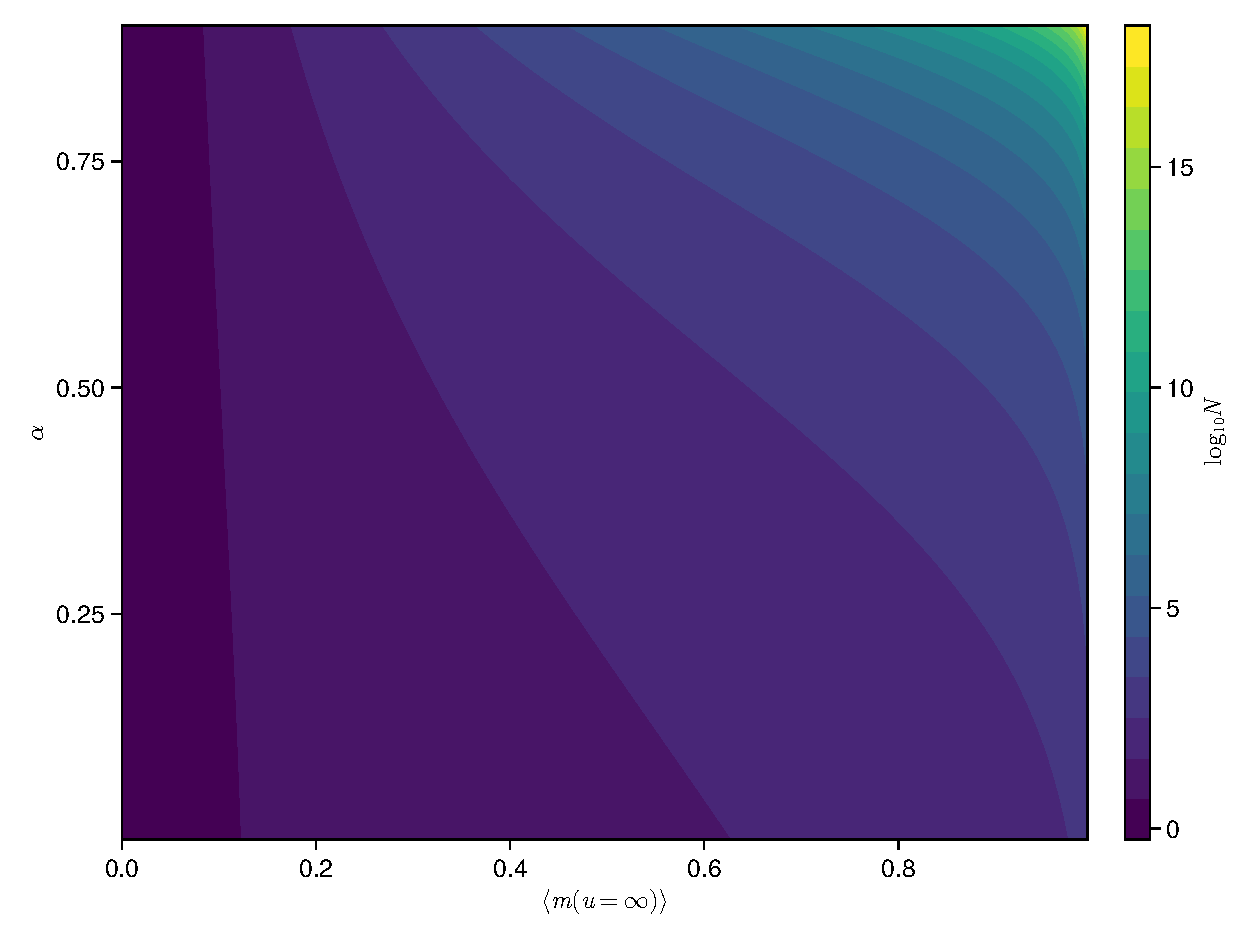
\includegraphics[width=.8\linewidth]{plots/N_formula_contour}
  \caption{\label{fig:N_formula_surface} \Cref{eq:19} evaluated for
    \(g_{0}^{2}=0.01\) and \(ω_{c}=1\).  For \(α\lesssim 4\) we can
    expect relatively good results for \(\ev{m}\) for
    \(\mathcal{O}(100)\) bath levels.}
\end{figure}


The expression \cref{eq:19} in monotonous in \(\abs{α_{A}}\) and thus
choosing an \(N\) such that \(\eval{ρ_{A}}_{α=α_{0}}\) implies that
\(\eval{ρ_{A}}_{{α}<α_{0}} \leq \eval{ρ_{A}}_{α=α_{0}}\).

Furthermore, at \(α\approx 1\) we can estimate
\(ζ(2-α)\approx 1/(1-α)\) and thus
\begin{equation}
  \label{eq:20}
  N \approx \pqty{ \frac{ω_{c}^{2}}{g_{0}^{2}}\pqty{\abs{α_{A}}^{-1}-1}\cdot
      \frac{1-α}{1+α}+1}^{\frac{1}{1-α}} \xrightarrow{α\to 1} \eu^{\frac{ω_{c}^{2}}{2g_{0}^{2}}\pqty{\abs{α_{A}}^{-1}-1}}
\end{equation}
showing that for the sharp phase diagram presented in
\refcite{Ricottone2020} exponentially many modes are required for a
fixed coupling strength. This is the origin of the finite size effects
on the \(α\) axis.

As for \(N\gg 1\) all discretization methods become equivalent, this
result is useful to estimate when \(N\) becomes prohibitively
large. In the case where \(N\sim 100\) or smaller using a different
density of states and the discretization methods described in
\cref{sec:discretization-bath} may pay off.



\subsection{Mean Displacement}
\label{sec:mean-displacement}

The results of \cref{sec:exact-solution,sec:criterion-bath-size} give
us the tools to construct finite-size systems to observe the effect of
a non-Markovian bath on the \ac{mlong}.

In general, the estimate \cref{eq:23} although being a lower bound for
the long time average of \(ρ_{A}\), can be beat by the instantaneous
value \(ρ_{A}(t)\) it reaches its minimum just before the revival time
due to the finite system size. This can happen, when optimizing for
the smallest number of bath levels \(N\) at a given coupling
strength. Thus it would be of advantage experimentally, to average
\(ρ_{A}\) over a time interval that excludes the revival and maybe
even the initial decay phase. In such cases \cref{eq:23} will
overestimate the number of required bath
levels. \Cref{fig:overview_shifted} highlights such a case. It will
therefore be useful to average \(\ev{m(t)}\) over a time interval of
\(\bqty{\frac{τ_{R}}{2}, \frac{9}{10} τ_{R} }\) where \(τ_{R}=2π N/ω_{c}\)
is the approximate time of the first recurrence.
\begin{figure}[ht]
  \centering
  \begin{subfigure}[t]{0.45\textwidth}
    \centering
    \includegraphics[width=\textwidth]{plots/overview_shifted.tikz}
    \caption{\label{fig:overview_shifted_many} With \(N=100\)
      bath levels. The mean displacement approaches the universal
      value for finite times and the infinite time limit is not
      too far off.}
  \end{subfigure}
  \begin{subfigure}[t]{0.45\textwidth}
    \centering
    \includegraphics[width=\textwidth]{plots/overview_shifted_few.tikz}
    \caption{\label{fig:overview_shifted_few} The same as
      \cref{fig:overview_shifted} but with \(N=8\) bath
      levels. Revivals shift the \ac{mlong} \(\ev{m}\) down.}
  \end{subfigure}
  \begin{subfigure}[t]{\textwidth}
    \centering
    \includegraphics[width=\textwidth]{plots/overview_shifted_few_windowed.tikz}
    \caption{\label{fig:overview_shifted_few_windowed} The same as
      \cref{fig:overview_shifted_few} but shown is the windowed time
      average value for \ac{mlong} and \(ρ_{A}\).  We see that this is
      a better extrapolation to the \(N\to ∞\) case. Further, the
      revivals are incomplete and interfere for different \(k\) values}
  \end{subfigure}
  \caption{\label{fig:overview_shifted} The same as
    \cref{fig:unshifted_overview} but with a shifted
    \(ω_{A}\). }
\end{figure}

The \(k\) dependence of the spectral density
\(J(ω) \sim {\abs{v(k)}^{2}}/{\abs{v(0)}} \) forces us to
choose a special \(k=0\) to calculate \(ω_{A}\). Here, we will choose
\(k=0\), as this makes \(ω_{A}\) independent of \(u\).

Further, as \(\abs{v(0)}\geq \abs{v(k\neq 0)}\) we will always choose
\(ω_{A}\) too big for all \(k\neq 0\). This generically leads to
\(ρ_{A}(k)\to 0\) decaying as \(U_{A}\) generically diverges
regardless of \(α\). However, this is not too problematic, as this
means that those \(ρ_{A}(k)\) simply don't contribute in the integral
\cref{eq:46}. On the other hand \(\abs{v(0)}\geq \abs{v(k\neq 0)}\)
can also lead to the effect, that the decay of \(ρ_{A}\) is slower for
\(k\neq 0\) than for \(k=0\). For \(u\approx 1\) there even are values
of \(k\) where \(v(k)\approx 0\) so that no decay takes place before
recurrence which will show up as a finite size effect and can be
witnessed in \cref{fig:transition_u_graphs.tikz}. However for \(u\)
sufficiently far from \(1\) this effect becomes minor. Also
\(\eval{∂_{k}\abs{v(k)}^{2}}_{k=0}=0\) so we have a non-vanishing
region where \(ω_{A}\) is chosen appropriately.


For \(u\ll 1\) or \(u\gg 1\) the amplitude
\(\abs{v(k)} \approx \abs{v(0)}\) so that we can use our estimate of
\(ρ_{A}(0)\approx ρ_{A}(k)\)
\begin{equation}
  \label{eq:34}
  \ev{m} \approx ∫_{0}^{2π} (1-ρ_{A}(0)) \dv{ϕ}{k}\frac{\dd{k}}{2π} =
  Θ(u-1)\,\pqty{1-ρ_{A}(0)},
\end{equation}
which is the \(\ev{m}\) value that the curve \(\ev{m}(u)\) will
saturate to. For \(u\gg 1\) we can replace
\begin{equation}
  \label{eq:55}
  \abs{α_{A}}=\sqrt{ρ_{A}}=\sqrt{1-\ev{m(u=∞)}}
\end{equation}
in \cref{eq:19} to estimate the number of bath modes required, where
\(\ev{m(u=∞)}\) is the desired value of the mean displacement.  As
mentioned above, this formula likely overestimates the required
\(N\) but may serve as a starting point.

Solving the full model with the \(B\) site preserved may alleviate
those ambiguities further and allow for the calculation of a berry
phase. The reduced model without the \(B\) site yields a purely real
Hamiltonian, as all phases can be absorbed into the basis
states. Therefore no nontrivial berry phase can arise.



\subsubsection{Decay Rate}
\label{sec:decay-rate}
The decay rate of \(ρ_{A}(k, t)\) can be estimated through the golden
(for a linear density of states) rule by setting local density of
states to \(ω_{c}/N\) and setting the squared matrix element to
\(J(ω_{A}) ω_{c}/N\)
\begin{equation}
  \label{eq:24}
  Γ=π\frac{N}{ω_{c}} J(ω_{A}) \frac{ω_{c}}{N} = π J(ω_{A}) =
  π (α+1)\frac{g_{0}^{2}}{ω_{c}} \pqty{\frac{ω_{A}}{ω_{c}}}^{α}.
\end{equation}

In the continuum limit and for \(α\to 0\) this becomes
\begin{equation}
  \label{eq:56}
  Γ = π \frac{g_{0}^{2}}{ω_{c}}
\end{equation}
which may be useful as a rough estimate for a minimal coupling strength.

Thus, averaging \(ρ_{A}\) over a time span between \(\approx 1/(2Γ)\)
and the recurrence time \(\approx 2π N / ω_{c}\) will make the phase
diagram sharper as is demonstrated in
\cref{fig:transition_u_graphs.tikz}.

Note that \(g_{0}^{2}\sim \abs{v(k)}^{2}\) so that \(Γ\) may not be
expected to give a very rigorous timescale but still might be useful
as an estimator. Numerically one can of course use the results of the
last section to reconstruct the full solution and get a more accurate
estimate.

Using \cref{eq:56} we can conclude that \(ω_{c}^{2}\)
\begin{equation}
  \label{eq:57}
  \frac{ω_{c}^{2}}{g_{0}^{2}} \lesssim N.
\end{equation}

\subsection{Phase Diagram}
\label{sec:phase-diagram}

With the results of \cref{sec:mean-displacement} we are finally in a
position to approximate the sharp phase diagram of
\cite{Ricottone2020} with finite coupling strength and a finite bath.

\Cref{fig:transition_u_graphs.tikz} shows the \(u\) dependence of the
\ac{mlong} for two values of \(α\) and a difference in behavior is
clearly visible. The full phase diagram can be seen in
\Cref{fig:fullphase}.
\begin{figure}[htp]
  \centering
  \includegraphics[width=.8\linewidth]{plots/transition_u_graphs_wider.tikz}
  \caption{\label{fig:transition_u_graphs.tikz} The \ac{mlong}
    averaged over an interval \([0.5τ, 0.95τ]\) where \(τ\) is the
    recurrence time. The coupling strength was \(g_{0}^{2}=.01\) and
    \(N=100\) bath levels were used. This is on the same order of
    magnitude of what \cref{eq:19} would suggest, but windowing
    improves the result.}
\end{figure}
\begin{figure}[htp]
  \centering
  \begin{subfigure}[t]{.49\linewidth}
    \includegraphics[width=\linewidth]{plots/phase_diag_100.tikz}
    \caption{With windowing.}
  \end{subfigure}
  \begin{subfigure}[t]{.49\linewidth}
    \includegraphics[width=\linewidth]{plots/phase_diag_100_nowindow.tikz}
    \caption{Without windowing. The phase diagram is slightly less
      crisp, but still acceptable.}
  \end{subfigure}
  \begin{subfigure}[t]{.5\linewidth}
    \includegraphics[width=\linewidth]{plots/phase_diag_100_nowindow_noshift.tikz}
    \caption{Without Lamb-Shift compensation. No universal values of
      \(\ev{m}\) are being reached.}
  \end{subfigure}
  \caption{\label{fig:fullphase}Full phase diagrams with the same
    parameters as \cref{fig:transition_u_graphs.tikz}.}
\end{figure}

It shall be noted that further optimizations are certainly
possible. For example, using an exponential density of states could
help for smaller \(N\).

\appendix
\section{Discretization of the Bath}
\label{sec:discretization-bath}
Given a subdivision of the energy axis \(\pqty{x_{i}}_{i\in [0,N]}\) with
\(x_{0}=0\) we would like to find coupling strengths \(η_{j}\) and energies
\(ω_{j}\) so
that
\begin{equation}
  \label{eq:26}
  ∫_{0}^{∞}f(ω)∑_{j}\abs{η_{j}}^{2} δ(ω-ω_{j})^{2}\dd{ω} =
  ∫_{0}^{∞}J(ω) f(ω) \dd{ω}
\end{equation}
for any smooth \(f(ω)\) in the limit \(N\to ∞\).
Discretizing \(f\) to be a linear combination of
\(f_{i}(ω)=Θ(x_{i}-ω) + Θ(ω-x_{i-1})\) (step function) we find
\begin{equation}
  \label{eq:27}
  η_{i}^{2} = ∫_{x_{i-1}}^{x_{i}}J(ω)\dd{ω} \approx J(ω) (x_{i}-x_{i-1}),
\end{equation}
where the second expression holds when \(x_{i}-x_{i-1}\ll ω_{c}\).

The choice of \(ω_{i}\) within \([x_{i-1}, x_{i}]\) is relatively
arbitrary, but one should avoid \(ω_{0}=0\) as this implies finite
coupling to a zero energy bath level. One method is to view \(J(ω)\) itself
as a distribution and choose~\cite{Bulla2003}
\begin{equation}
  \label{eq:28}
  ω_{i} =
  \frac{∫_{x_{i-1}}^{x_{i}}J(ω)ω\dd{ω}}{∫_{x_{i-1}}^{x_{i}}J(ω)\dd{ω}}
  = η_{i}^{-2} ∫_{x_{i-1}}^{x_{i}}J(ω) ω\dd{ω}.
\end{equation}

Another approach is the postulate a density of frequencies \(ρ_{f}\)
with \(\int_{0}^{∞}ρ_{f}(ω) \dd{ω} = 1\)
and choose the discretization of the frequency axis accordingly
\begin{equation}
  \label{eq:29}
  ∫_{0}^{x_{i}} ρ_{f}(ω) \dd{ω} = \frac{i}{N}
\end{equation}
where \(N\) is the number of bath levels. Then one can choose the
\(ω_{i}\) according to this distribution
\begin{equation}
  \label{eq:30}
  ω_{i} =
  \frac{∫_{x_{i-1}}^{x_{i}}ρ_{f}(ω)ω\dd{ω}}{∫_{x_{i-1}}^{x_{i}}ρ_{f}(ω)\dd{ω}}
\end{equation}
or to the median with respect to this distribution~\cite{Hartmann2019}
\begin{equation}
  \label{eq:31}
  ∫_{0}^{ω_{i}} ρ_{f}(ω) \dd{ω} = \frac{i-1}{N} + \frac{1}{2N} = \frac{2i-1}{2N}.
\end{equation}

An advantage of the latter choice is, that it prevents \(ω_{0}=0\) and
is easier to compute than \cref{eq:30}, as \cref{eq:29} can be reused.


The choice of \(ρ_{f}=1/ω_{c}\) yields together with \cref{eq:49}
\begin{equation}
  \label{eq:33}
  \begin{aligned}
    x_{i} &= ω_{c}\frac{i}{N} & ω_{i} &= ω_{c} \frac{2i-1}{2N} & η_{i}^{2}
    &= ∫_{ω_{c}\frac{i-1}{N}}^{ω_{c}\frac{i}{N}}J(ω)\dd{ω} = \frac{g_{0}^{2}}{N^{α+1}} \pqty{i^{α+1}-(i-1)^{α+1}}.
  \end{aligned}
\end{equation}

The values \cref{eq:33} are used for the exact diagonalization in the
preceding sections.  For analytic calculations it is easiest to choose
\(ω_{i} = x_{i}\) along with replacing the integral \cref{eq:27} with
\(η_{j}^{2} = {g_{0}^{2}(α+1)} j^{α}/N^{α+1}\) and \(ω_{j}=jω_{c}/N\)
which is the limit of \cref{eq:33} for \(N\gtrsim 100\).

Another choice of for the energy level distribution is \(ρ_{f} =
Δ^{-1} \eu^{-\frac{ω}{Δ}}\) which emphasizes the structure of the bath
at \(ω\approx 0\). The parameter \(Δ\) is arbitrary, but when using an
exponential cutoff for the spectral density
\begin{equation}
  \label{eq:50}
  J(ω) = \tilde{J}_{α} ω^{α} \eu^{-\frac{ω}{ω_{c}}}= \frac{g_{0}^{2}}{ω_{c}^{1+α}Γ(1+α)} ω^{α} \eu^{-\frac{ω}{ω_{c}}},
\end{equation}
it is natural to set \(Δ=ω_{c}\).
With this we obtain
\begin{equation}
  \label{eq:51}
  \begin{aligned}
    x_{i} &= -ω_{c} \ln(1-\frac{i}{N}) & ω_{i} &= -ω_{c} \ln(1-\frac{2i-1}{2N}).
  \end{aligned}
\end{equation}
The coupling constants \(η_{i}\) can be determined by evaluating the
antiderivative of \cref{eq:50}
\begin{equation}
  \label{eq:52}
  \mathcal{J}(ω) = -ω^{α+1}
  \frac{E_{-a}\pqty{\frac{ω}{ω_{c}}}}{ω_{c}^{α+1} Γ(α+1)},
\end{equation}
where \(E_{n}(z)=∫_{1}^{∞}\eu^{-zt}/t^{n}\dd{t}\) is the exponential
integral.


Whether to replace the integral in \cref{eq:50} by a multiplication
depends on the number of reservoir levels and the choice of the \(ω_{i}\). When
choosing the energies according to \cref{eq:51}, then
\cref{fig:mean_displacement_benchmark} shows that
we get away with multiplication.

\begin{figure}[p]
  \centering
  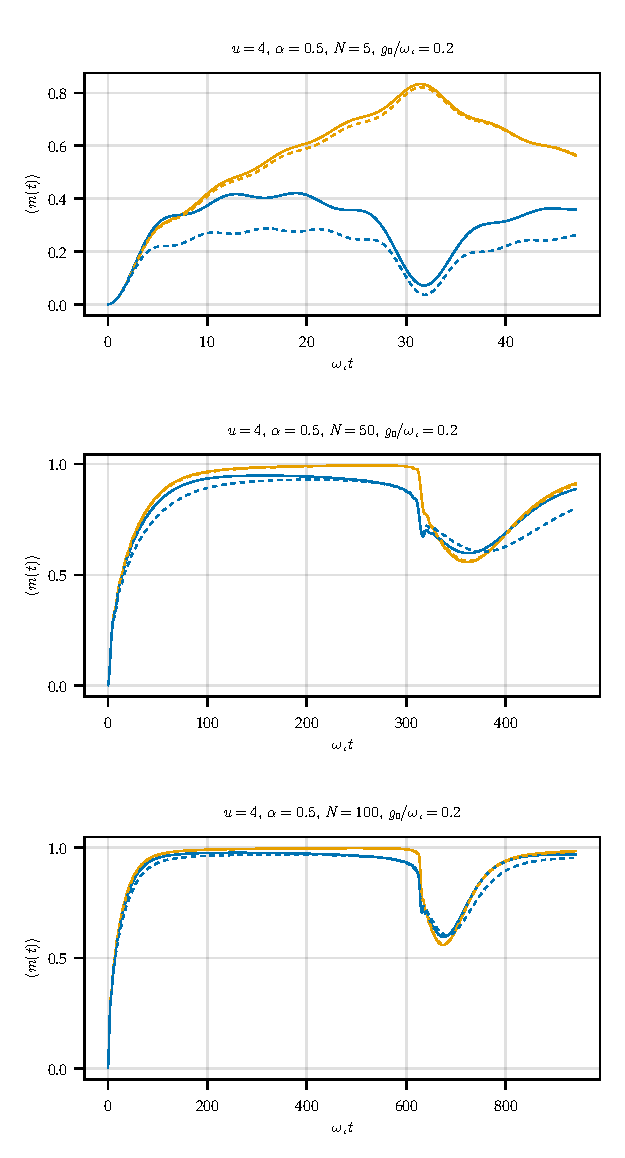
\includegraphics{plots/mean_displacement_complicated_vs_simple_energy}
  \caption{\label{fig:mean_displacement_benchmark} The mean
    displacement for multiple reservoir sizes. The blue lines
    correspond to choosing the energies \(ω_{j}=x_{j}=ω_{c} j/N\)
    whereas the blue lines use \cref{eq:51}. The solid lines use
    integration and the dashed lines use multiplication in \cref{eq:50}.}
\end{figure}


\section{Recipe for Obtaining the Phase Diagram}
\label{sec:recipe-obta-phase}
This section gives a condensed overview of how to choose the model
parameters. A worked example is provided along with plots of the
results.  Throughout we choose \(ω_{c}=1\) but still include it in the
formulas. The parameter \(v\) in the model \cref{eq:37} becomes
redundant due to the choice of the normalization of the spectral
density and can be set to unity.

\subsection{Discretization of The Bath}
\label{sec:discretization-bath-1}
The simplest choice is
\begin{equation}
  \label{eq:53}
  \begin{aligned}
    x_{i} &= ω_{c}\frac{i}{N} & ω_{i} &= ω_{c} \frac{2i-1}{2N} & η_{i}^{2}
    &= J(ω_{j}) \frac{ω_{c}}{N}
  \end{aligned}
\end{equation}
% \begin{equation}
%   \label{eq:32}
%   \begin{aligned}
%     ω_{j} &= ω_{c}\frac{j}{N} & η_{j}^{2} = J_{α} ω_{j}^{α}
%                                 \frac{ω_{c}}{N} = \frac{\abs{v(k)}^{2}}{\abs{v(0)}^{2}}\,{g_{0}^{2}(α+1)} \frac{j^{α}}{N^{α+1}}
%   \end{aligned}
% \end{equation}
where \(v(k)= v+v' \eu^{\iu k} = v (1+u \eu^{\iu k})\) and should be
sufficient. For more elaborate constructions and more background
information see \cref{sec:discretization-bath}.

\subsection{Coupling Strength and Number of Bath States}
\label{sec:coupling-strength}

The general requirement is that\footnote{See
  \cref{sec:mean-displacement,sec:exact-solution}}
\(N^{-1}ω_{c}^{2} \lesssim g_{0}^{2}\ll ω_{c}^{2} (α + 1) \). On the
other hand, one does not want the dynamics to be too slow so that
revivals occur too soon. Therefore we pick a coupling strength so that
the aforementioned condition is fulfilled with a reasonable number of
bath modes.

We then evaluate
\begin{equation}
  \label{eq:54}
  N = \bqty{\pqty{\frac{ω_{c}^{2}}{g_{0}^{2}}\frac{\frac{1}{\sqrt{1-\ev{m}}}-1}{(α+1)}+\frac{1}{1-α}}\frac{1}{ζ(2-α)}}^{\frac{1}{1-α}}
\end{equation}
to see if it matches the order of magnitude of bath modes that can be
achieved experimentally for an \(α\lesssim 1/2\). Here \(\ev{m}\) is
the desired long time average of the mean displacement at a specific
\(α\) for \(u\to ∞\).  The choice of \(α\) in this formula specifies,
where one would like to have universal values for the phase transition
as a function of \(u\). If \cref{eq:54} doesn't match the order of
magnitude of the first estimate of \(N\), the desired \(\ev{m}\) has
to be reconsidered (lowered). Alternatively the sharpness of the phase
transition on the \(α\) axis can be lowered by choosing a lower \(α\)
in the above.


For concreteness, let us choose \(α=0.1\) and \(g_{0}^{2}=0.01\) and
\(\ev{m}=.8\). The choice of the mean displacement relatively far from
\(1\) is made in the expectation that a windowed average will improve
it, as \cref{eq:54} only take the infinite time average into account
which will be less because of revivals.  The above estimate
\cref{eq:54} then yields \(N=104\) which is consistent with
\(N^{-1}\lesssim g_{0}^{2}\). \Cref{fig:n_lim_ex} shows of the lower
bound on \(N\) for a range of \(\ev{m}\) and \(g_{0}^{2}\).
\begin{figure}[H]
  \centering
  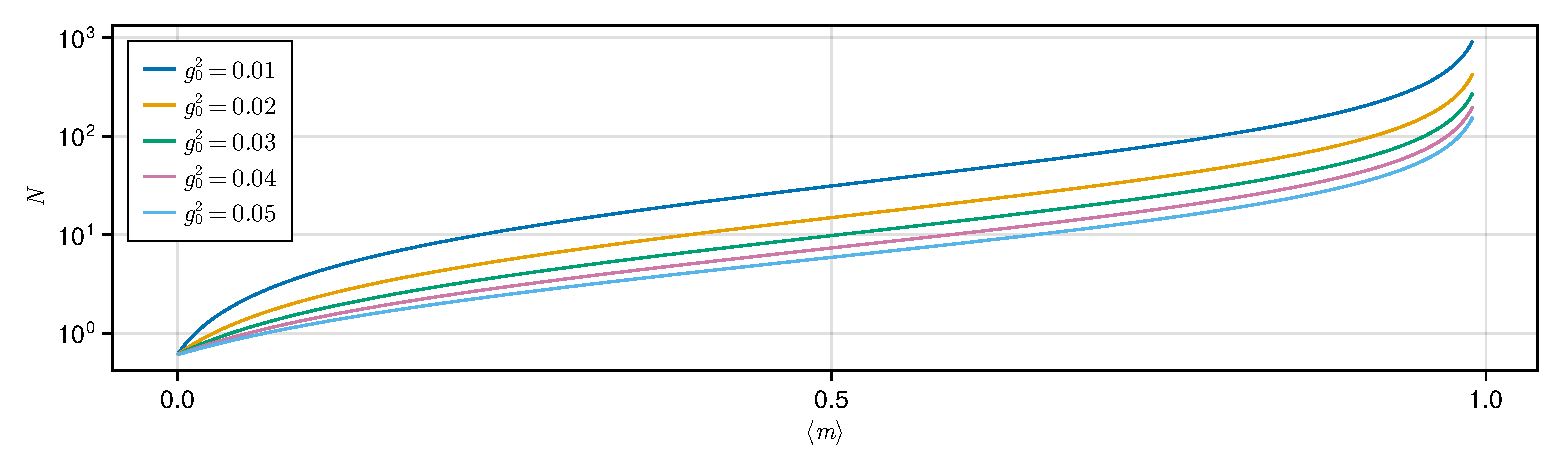
\includegraphics[width=\linewidth]{plots/example_N_limits}
  \caption{\label{fig:n_lim_ex} \cref{eq:54} evaluated for different
    coupling strengths.}
\end{figure}

\subsection{Refining the Parameter Choices with Numerics}
\label{sec:refin-param-choic}

Once the parameters are chosen according to
\cref{sec:coupling-strength}, numerics can be used to refine the
parameter choices, as all of the above is based on rough estimates.

A starting point would be to plot slices of constant \(α\) through the
phase diagram, for the \(α\) chosen in \cref{sec:coupling-strength}
and one that is larger than one. Adjustments of \(N\) and
\(g_{0}^{2}\) may then be made to obtain the desired behavior with as
few bath modes as possible. The \(α<1\) curve should saturate to zero
and one for \(u\to 0\) and \(u\to ∞\) respectively with the sharpness
of the transition being dependent on \(N\), whereas the \(α>1\) curve
should saturate at a non-universal value.
\begin{figure}[H]
  \centering
  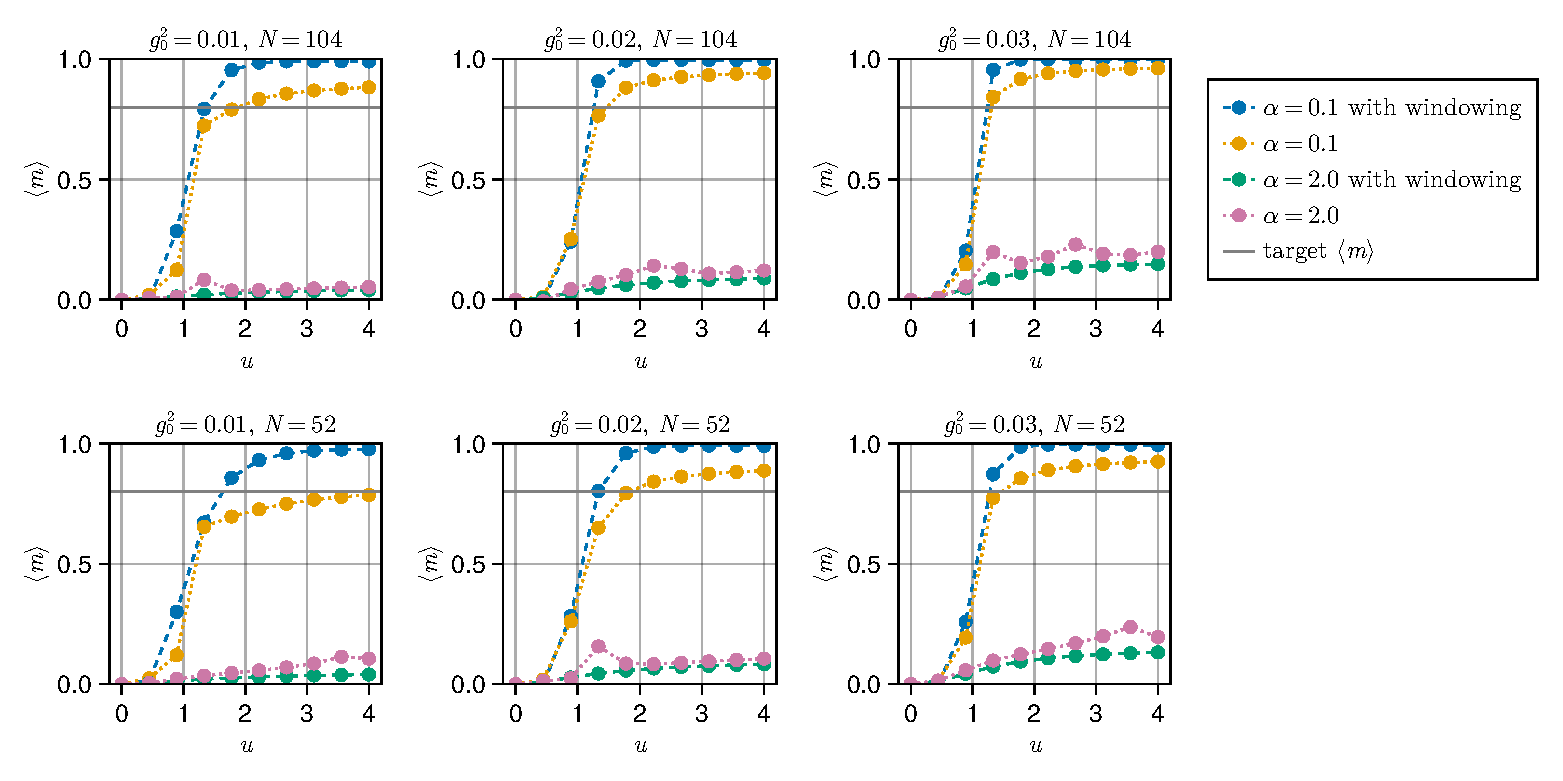
\includegraphics[width=\linewidth]{plots/example_cuts}
  \caption{\label{fig:example_cuts} The \ac{mlong} \(\ev{m}\)
    evaluated by exact diagonalization for multiple values of \(u\)
    and \(α\) with and without windowing of the average. The original
    target \(\ev{m}\) that was used in \cref{eq:54} is also shown.}
\end{figure}

To counter the effect of recurrences, the time average of \(\ev{m}\)
should be taken over an interval
\(\bqty{\frac{τ_{R}}{2}, 0.95 τ_{R} }\) where \(τ_{R}=2π N/ω_{c}\) is
the approximate time of the first recurrence. These interval
boundaries are a starting point and can be altered if desired.

\Cref{fig:example_cuts} shows such a set of slices for different
parameter choices. It is evident, that windowing the average does
increase the sharpness of the phase diagram cuts.  further, we can see
that if we allow for relatively large \(u\), we find
\(\ev{m}\approx 1\) for \(u>2\) even for half the number of bath
levels, if we double the coupling strength \(g_{0}^{2}\), although the
best sharpness is obtained for \(N=104\) and \(g_{0}^{2}=0.03\).

Using those values, we may plot the full phase diagram in \cref{fig:example_full_diag}.
\begin{figure}[H]
  \centering
  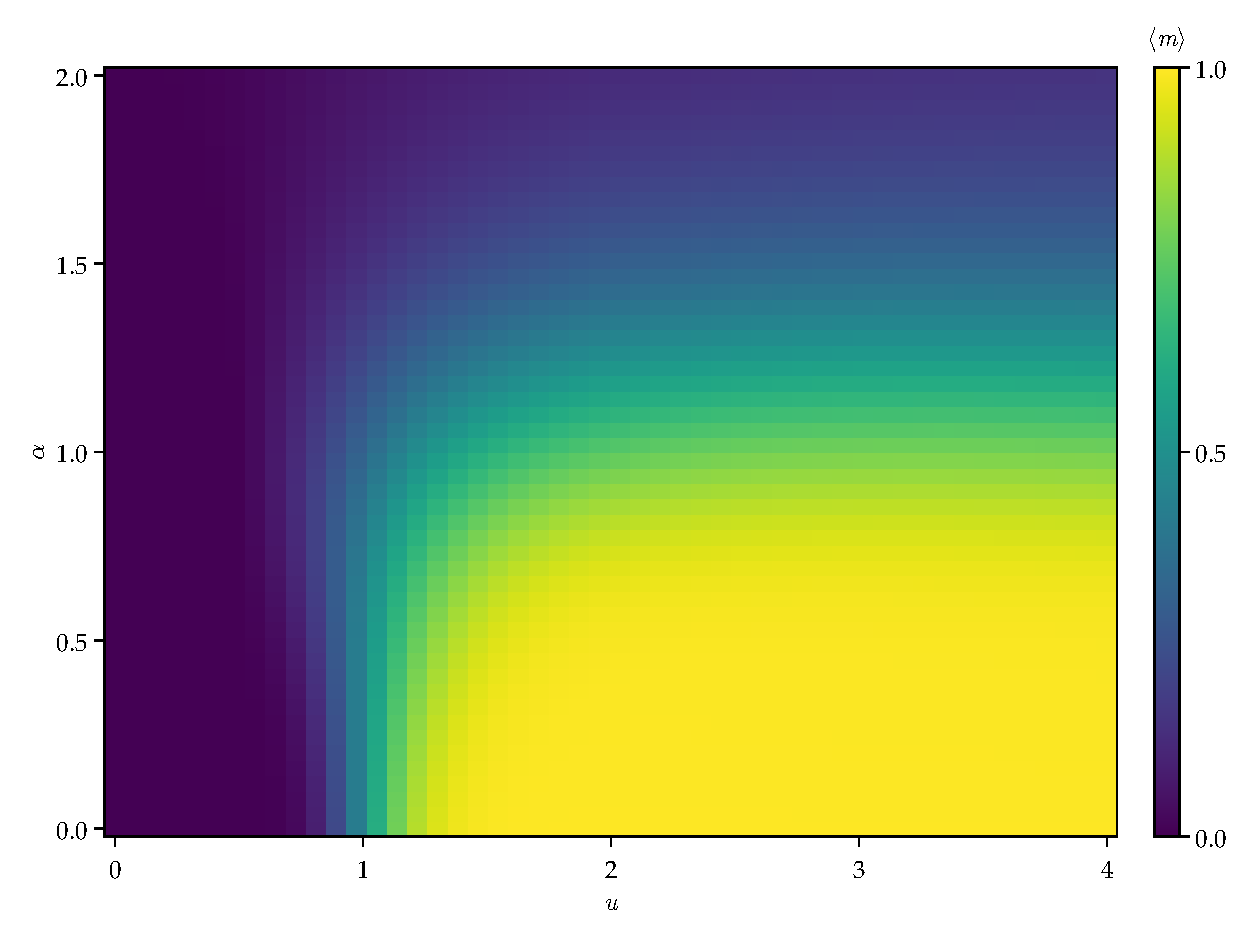
\includegraphics[width=.8\linewidth]{plots/example_full_diag}
  %\includeplot[scale=.5,width=\linewidth]{example_full_diag}
  \caption{\label{fig:example_full_diag} The full phase diagram for
    \(N=100\) bath modes and \(g_{0}^{2}=0.03\) using the windowed
    average.}
\end{figure}

\printbibliography{}
\printacronyms{}
\end{document}


%%% Local Variables:
%%% mode: latex
%%% TeX-master: t
%%% TeX-output-dir: "output"
%%% TeX-engine: luatex
%%% End:
